\documentclass[conference]{IEEEtran}
\IEEEoverridecommandlockouts
\usepackage{cite}
\usepackage{amsmath,amssymb,amsfonts}
\usepackage{algorithmic}
\usepackage{graphicx}
\usepackage{textcomp}
\usepackage{xcolor}

\def\BibTeX{{\rm B\kern-.05em{\sc i\kern-.025em b}\kern-.08em
    T\kern-.1667em\lower.7ex\hbox{E}\kern-.125emX}}

\title{Surface Crack Detection via Deep Learning\\
{\footnotesize \textsuperscript}
}
\makeatletter
\newcommand{\linebreakand}{%
  \end{@IEEEauthorhalign}
  \hfill\mbox{}\par
  \mbox{}\hfill\begin{@IEEEauthorhalign}
}
\makeatother

\author{
\IEEEauthorblockN{Catherine Cho}
\IEEEauthorblockA{\textit{Applied Data Science of SJSU
} \\
catherine.cho@sjsu.edu}
\and
\IEEEauthorblockN{Jie Hu}
\IEEEauthorblockA{\textit{Applied Data Science of SJSU
} \\jie.hu@sjsu.edu}
\and
\IEEEauthorblockN{Dahlia Ma}
\IEEEauthorblockA{\textit{Applied Data Science of SJSU
} \\dahlia.ma@sjsu.edu}
\linebreakand 
\IEEEauthorblockN{Ashima Malik}
\IEEEauthorblockA{\textit{Applied Data Science of SJSU
} \\ashima.malik@sjsu.edu}
\and
\IEEEauthorblockN{Tanyu Yin}
\IEEEauthorblockA{\textit{Applied Data Science of SJSU
} \\ tanyu.yin@sjsu.edu}
}

\begin{document}
\maketitle

\begin{abstract}
Currently, the majority of infrastructures use concrete material. So the quality of concrete structures are important as they can affect the safety, durability, and applicability of the structure. Due to the material being susceptible to cracks, it is necessary to inspect the rigidity and tensile strength of the buildings to prevent them from catastrophic collapsing events. However, manual human inspection is time consuming, tedious, and costly. Therefore, there have been several past studies that have utilized deep learning techniques such as convolutional neural networks (CNN) to automate the process of detecting surface cracks. In this project, performance of six different deep learning models used in previous studies were to determine the accuracy and efficiency of surface crack detection. Results show that all models achieved good test accuracy of at least 95 percent, and proved that shallower neural networks with less memory requirements can perform as well as deeper neural networks with the dataset used in this project. 
\end{abstract}

\section{Introduction}
Concrete structure accounts for the largest proportion in present infrastructure builds. Although concrete infrastructure has good rigidity and tensile strength, they also encounter cracks frequently. If these cracks are not identified and treated timely, they can cause serious safety and durability issues in buildings and infrastructures. Statistical analysis reveals that almost 46 percent of the weakness in structures or buildings is due to the failure of detecting structural cracks [1]. Therefore, it is crucial to detect structural cracks in a timely manner, and take the required maintenance measures for the safety of buildings. Traditional manual methods to detect cracks are taxing and time consuming, but it also has substantial unseen dangers to workers safety. Hence, a myriad of research has been using machine learning and deep learning methodologies to find efficient ways to detect surface cracks using digital applications. Several research has provided satisfactory results to overcome the several limitations of manual detection, proving that deep learning techniques can handle large amounts of image data while automating feature extraction processes to detect surface cracks. Moreover, several studies have proposed different optimized individual neural networks to detect surface cracks, but no studies have made performance comparisons of all these individual neural networks. So the goal of this project was to compare the performance and memory requirements of the following six models: VGG-16, ResNet50, MobileNet, CNN, LeNet5 and OLeNet, using accuracy and parameter numbers as the evaluation criteria.
\section{Literature Survey}
Much research has been done using various edge detection algorithms such as the wavelet method and Laplace of Gaussian to detect the cracks [2]. Abdel- Qader et al. compared four different edge detection methods such as Haar transform, fast Fourier transform, Sobel, and Canny. However, results did not show promising results in terms of accuracy [3]. Researchers have also used standard machine learning algorithms such as K-means clustering and Support Vector Machines (SVM) to detect surface cracks, but such algorithms were not successful in processing large volumes of image data [4]. Hence, deep learning techniques have been deployed in computer vision, pattern recognition, and object detection. Convolutional Neural Networks (CNNs) have demonstrated the capability to relate the complex input and output relationship using nonlinear activation functions, and it also handles large volumes of data well while automating feature extraction. Past studies have optimized different CNN models such as ResNet, AlexNet, VGG-16 to identify the cracks. VGG-16 is a commonly used pretrained model that deeply stacks with 16-layer depth, ResNet has a depth of 152 layers, and Inception has a depth of 159 layers with a parallel stacked convolutional network. Although deep networks such as these extract more features from images and are prone to overfitting with smaller datasets. A study on pavement distress detection from Seichter et al. [6] constructed a VGG-inspired deep neural network called ASINVOS net to automate the detection of pavement cracks. The ASINVOS net was a convolutional neural network that consisted of a total of eight convolutional layers, three max-pooling layers, and three fully connected layers. Each layer in the ASINVOS network used ReLU as the activation function except for the last layer, and dropout was added to every hidden layer to regularize the model, as the model had a total of approximately 4 million parameters [6]. Results of [6] showed that the ASINVOS net had a F1 score of about 87 percent on the test set with this architecture. Another study, Cha et al [7] used CNN to detect the crack damage in concrete walls where the network was trained with 40,000 images of 256 x 256 pixel resolutions, and achieved 98 percent accuracy in crack detection on validation set. In a recent 2021 study [9], an optimized LeNet5 model called OLeNet was proposed for better performance while preserving shallow depth in architecture with less memory requirements. The study [9] compared OLeNet to VGG-16, ResNet, and Inception, and results showed OLeNet achieved high accuracy of at least 99 percent as the rest of the deeper networks, with the exception that ResNet only achieved 97.0 percent accuracy. 
\section{Methodology}
\subsection{Data Collection and Preprocessing}
The dataset was available to the public and provided by METU. The dataset was generated from 458 high-resolution images that contained different concrete surface images proposed by [8]. There were 20,000 positive and 20,000 negative images with 227 x 227 pixels with RGB channels, in which positive images had cracks and negative images did not. And no preprocessing was required as all images were the same size. 
Unlike previous studies, the original dataset was augmented by adjusting brightness between the range of 0.2 to 0.6, and flipping images by 90 degrees with horizontal flip. The brightness adjustment accounted for different luminations, and the flipping accounted for different crack positions. Each image produced nine augmented images. As a result, there were a total of 400,000 positive and negative augmented images. 
\begin{figure}[htbp]
\centerline{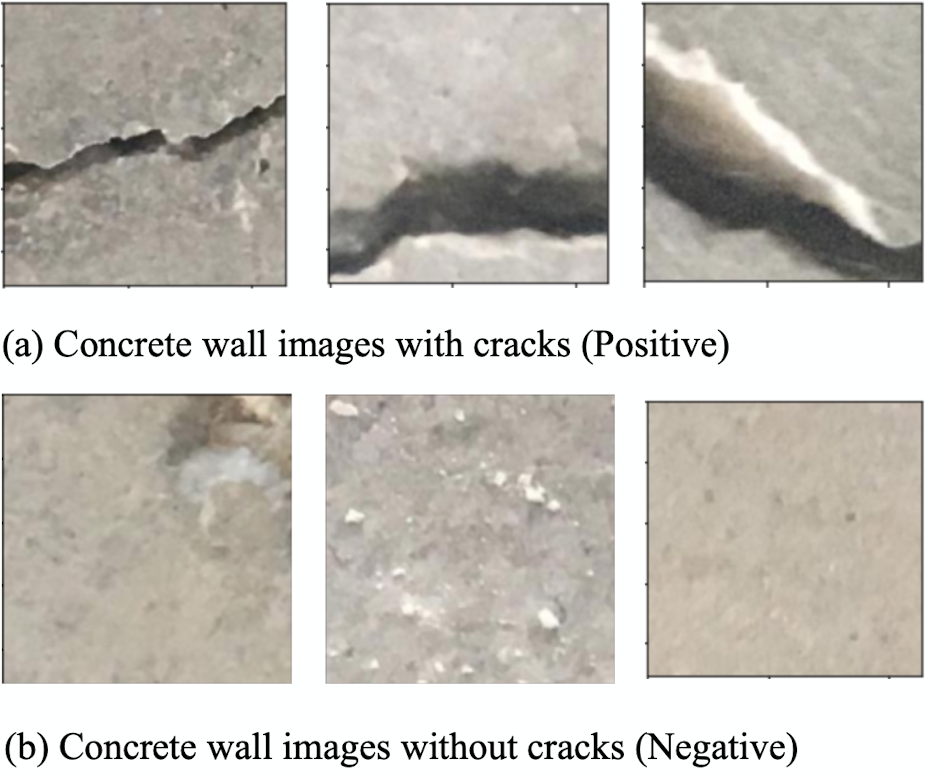
\includegraphics[scale=0.45]{Fig1_image_example.png}}
\caption{Image Datasets Example}
\label{table}
\end{figure}
\subsection{Architectures}
\subsubsection{VGG-16} \\
The VGG-16 network consisted of two sets of two convolutional layers followed by max pooling, and three sets of three convolutional layers followed by max pooling. A flatten layer followed along with two fully connected (FC) layers. The first FC layer had 64 neurons and the second FC layer had two neurons with softmax activation function. All layers with learnable parameters, except for the last, used ReLU as the activation function. The initial number of epochs to train was set to 25, but with early stopping of a patience of 1, the model converged at 8 epochs. The learning rate was set at 0.01, and the loss method used was categorical cross entropy with the Adam optimizer.
\subsubsection{ResNet50}
The ResNet50 model is a popular deep residual network for image recognition, which is also a type of convolutional neural network. ResNet50 is a variant of the ResNet model that contains 50 layers in depth, which has 48 convolutional layers along with one max pool layer and one average pool layer. The model contained five different stages where each stage had a residual block, and each residual block consisted of three layers with both 1x1 and 3x3 convolutions, resulting in over 23 million trainable parameters. With residual blocks, identity connections are formed where each layer feeds directly into the next two to three layers. The initial number of training epochs was set to 100, but with early stopping with a patience of 1, the model converged at 3 epochs with a batch size of 64. Within the model architecture, a learning rate of 0.001 with the Adam optimizer was incorporated, and the categorical cross entropy was used as the loss method.
\subsubsection{MobileNet}
The MobileNet was a neural net proposed by Andrew G. Howard et al of Google Research team [10]. MobileNet was built on depth-wise separable convolutions, except for the first layer in which is a full convolutional layer. All layers in the network are followed by the batch normalization and ReLU non-linearity. However, the final layer is a fully connected layer without any non-linearity and feeds to the softmax for classification. For down-sampling, strided convolution was used for both depthwise convolution and the first full convolutional layer. The network had a total of 28 layers including depthwise and pointwise convolution as separate layers. The model was trained over 10 epochs with a batch size of 16, using the Adam optimizer with a learning rate of 0.0001, and the loss method used was categorical cross entropy
\subsubsection{CNN}
Convolutional Neural Network (CNN) is a common class of neural networks used to analyze and classify images. This project created and experimented with an improvised CNN where there were more fully connected layers than convolutional layers. The improvised CNN model contained three convolutional layers with each layer followed by max pooling. A flatten layer was included between the last convolution layer and five fully connected layers (with different numbers of neurons). In every layer with learnable parameters, except for the last, ReLU was used as the activation function. The optimized hyperparameters for this model include a learning rate of 0.01, the binary cross entropy as the loss method, and the Adam optimizer, trained for 10 epochs.
\subsubsection{LeNet5}
LeNet5 is a shallow 5-layer CNN proposed by LeCun in 1998. This model served as a reference for the OLeNet model. During development, a batch size of 64 was used for model training. This network has five layers with learnable parameters consisting of three convolutional layers followed by an average pooling layer each, and two fully connected layers ending with softmax. With the exception of the last layer before softmax, ReLU was the activation function for each layer. The optimized hyperparameters for LeNet5 used a learning rate of 0.001, the cross entropy loss method, the Adam optimizer, and trained for 7 epochs. During modeling, learning rates of 0.1 and 0.01 were attempted but both learning rates were too large for loss performance to improve. As the original model proposal used a tanh activation, this was compared to the performance of using the ReLU activation. In comparison, ReLU achieved 99.4 percent validation accuracy at 7 epochs while tanh achieved 95.9 percent accuracy at 6 epochs.
\subsubsection{OLeNet}
As mentioned previously, the OLeNet model is an optimized version of LeNet5. Unlike LeNet5, the OLeNet has two extra convolutional layers, where two convolutional layers were stacked together followed by max pooling and dropout for better generalization. The final architecture used SeLU instead of ReLU as the activation function, as it performed better in accuracy and training time. A batch size of 64 was used during training, and the final model was optimized with a learning rate of 0.001, the cross entropy loss method, the Adam optimizer, and converged at 4 epochs. As the original proposal of OLeNet used ReLU as the activation function, SeLU was also explored as an option. Results showed that SeLU trained twice as fast than using ReLU, and SeLU achieved identical validation accuracy of 99.4 percent as using ReLU.
\subsection{Evaluation Methods}
To evaluate the models, accuracy was used to measure surface crack detection performance. Accuracy was calculated as the total number of correct detections divided by the total number of images detected. Furthermore, the total number of parameters was also used as a criterion to provide more memory requirements context to model performance. Due to limited time constraints and computing resources, it was not possible to train the models with 400,000 augmented data as it took approximately four days for one variation of LeNet5 to reach minimum loss. Hence, 1,000 of the augmented images were used to further evaluate test accuracy of each model.
\section{Results}
As shown in Figure 2 (a), the training accuracy for VGG-16 already started with high accuracy in epoch 1. The model started plateauing around epoch 4, and converged at around 8 epochs. Overall, the training accuracy was 99.95 percent and the validation accuracy was 99.78 percent. The test accuracy with the non-augmented or original data was 99.96 percent, and the test accuracy using augmented images was 99.93 percent. Similarly, shown in Figure 3 (a), the training loss significantly improved around epoch 1 (which is also the second epoch). Both VGG-16 loss and accuracy graphs show that validation results consistently slightly beat those of training; the training loss with non-augmented dataset was 0.0015, and the validation loss was 0.0011. This indicates that the VGG-16 model was underfitting as the validation set performed better than the training set.
Figure 2 (b) shows that the ResNet50 model reached training and validation accuracies higher than 99.90 percent. Model training was stopped early at the third epoch as it reached a 99.92 percent and 99.90 percent training and validation accuracy, respectively; so training was stopped so the model would not continue to overfit. The test accuracy with non-augmented data was 99.79 percent and 96.10 percent with augmented data. At convergence, the training and validation losses were as low as 0.0025. Unlike the other models, ResNet50 experienced an interesting phenomenon where the validation set performed better than the training set before the third epoch, however started overfitting afterwards.
Continuing onto MobileNet, training accuracy improved from 98.35 to 99.94 percent, and validation accuracy improved from 99.7 to 99.95 percent during training. The test accuracy using non-augmented test data was 99.91 percent, and 97.60 percent using augmented data. As shown in Figure 3 (c), the MobileNet model improved in loss over time and converged at epoch 10. At epoch 10, the loss values for training and validation were 0.0022 and 0.0019, respectively. Similar to VGG-16, both loss and accuracy graphs indicate that the MobileNet may be underfitting as there was no healthy gap between the training and validation sets.
For the improvised CNN, figure 2 (d) shows that both training and validation accuracies overlapped and achieved higher than 98 percent. As shown in figure 2 (d), training accuracy improved from less than 90 percent to above 98 percent in epoch 2 (or the third epoch if started epoch count at 1). Comparable to the accuracy graph, figure 3 (d) shows similar improvement patterns in training loss, but with slightly more volatility. At convergence, the validation loss and accuracy were 0.1136 and 98.37 percent, respectively. As illustrated in both loss and accuracy plots, the validation set performed either the same or slightly better than the training set indicating that the improvised CNN model may be underfitting.
Moving onto a shallower network, LeNet5, figure 2 (e) and 3(e) show that both training and validation accuracy and loss were similar and overlapped. After the second epoch of training, both training and validation achieved accuracies higher than 95 percent. In terms of loss, shown in figure 3 (e), both training and validation loss significantly improved at the second epoch, from 90 to at least 97 percent. The LeNet5 model reached minimum loss at around epoch 7, with a training and validation loss of 0.020 and 0.018, respectively. 
In comparison to LeNet5, figure 2 (f) shows that the OLeNet model exhibited slower improvement in training and validation accuracies between epochs 1 and 3. Figure 2 (f) shows that OLeNet with SeLU activation maintained steady accuracy until epoch 9. At epoch 10, a strange phenomenon occurred where the training accuracy abruptly dropped to 86 percent. It turns out that a quarter of the middle iterations in epoch 10 were experiencing low training accuracies between 40 and 60 percent. The reason for such an occurrence is unknown, but it may be possible that the model was fitting to noise to an extent that resulted in the lower accuracy; as it is not possible for the model to experience vanishing or exploding gradient since it was using SeLU as the activation function, in which it has a self-normalization mechanism. Like the accuracy graph, the loss graph shown in figure 3 (f) shows mirroring trends where the training loss dramatically increased from less than 0.05 to almost 0.35 at epoch 10. Overall, the OLeNet model performed similarly as the LeNet5 reference model in terms of accuracy where both models achieved 99.38 percent in validation accuracy. However, OLeNet outperformed LeNet5 in terms of training speed where OLeNet converged in half the epochs than LeNet5. Despite the high accuracies and low losses in LeNet5 and OLeNet, both models did not exhibit a healthy gap which may indicate underfitting.

\begin{figure}[htbp]
\centerline{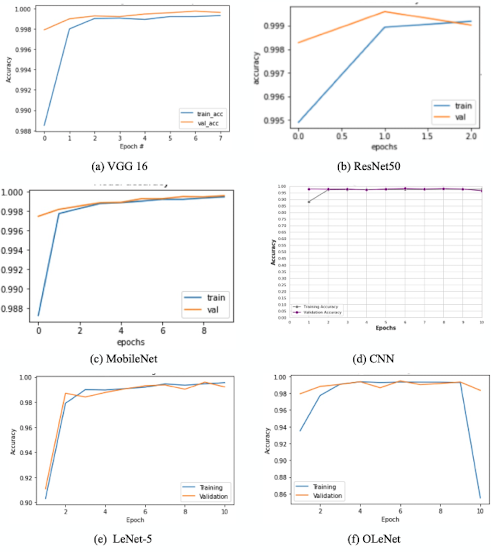
\includegraphics[scale=0.45]{Fig2_accuracy_plot.png}}
\caption{Models Training/Validation Accuracy}
\label{fig}
\end{figure}
\begin{figure}[htbp]
\centerline{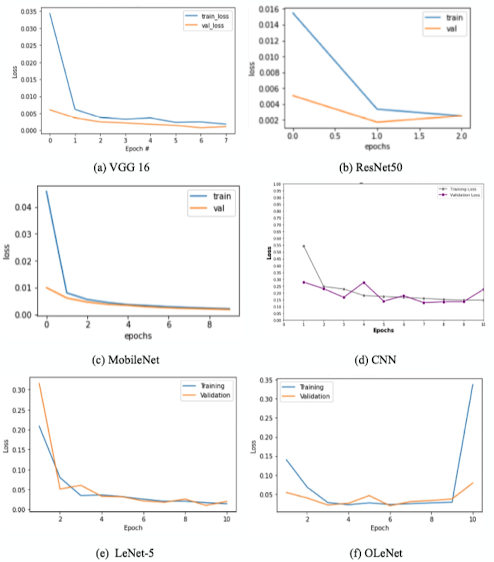
\includegraphics[scale=0.50]{Fig3_loss_plot.png}}
\caption{Models Training/Validation Loss}
\label{fig}
\end{figure}
\begin{figure}[htbp]
\centerline{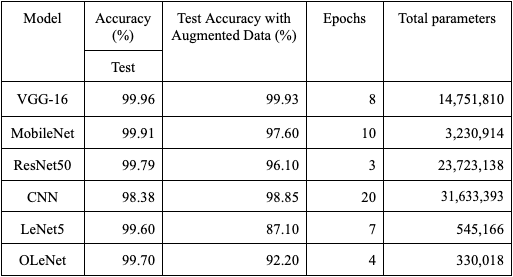
\includegraphics[scale=0.45]{Fig4_table.png}}
\caption{Summary Table: Test Accuracy with non-augmented and augmented dataset}
\label{table}
\end{figure}
As mentioned in previous sections, all models were trained with the non-augmented original dataset, and test accuracy was measured using both original and augmented datasets. Due to the enormous volume of the augmented dataset, only 1,000 randomly selected augmented images were used to further evaluate test accuracy for each model. Figure 5 demonstrates that VGG-16 consistently outperformed all other models in both non-augmented and augmented test accuracies, and LeNet5 performed the worst. Unlike the rest, the improvised CNN model achieved slightly better accuracy with augmented images than that of non-augmented images. Interestingly, the summary table shown in figure 4 shows that the performance of MobileNet was almost on par with that of VGG-16 with a fifth of VGG-16’s total number of parameters. And OLeNet only performed about 5 percentage points worse than MobileNet in augmented test accuracy with only a tenth of MobileNet’s total number of parameters. 

\begin{figure}[htbp]
\centerline{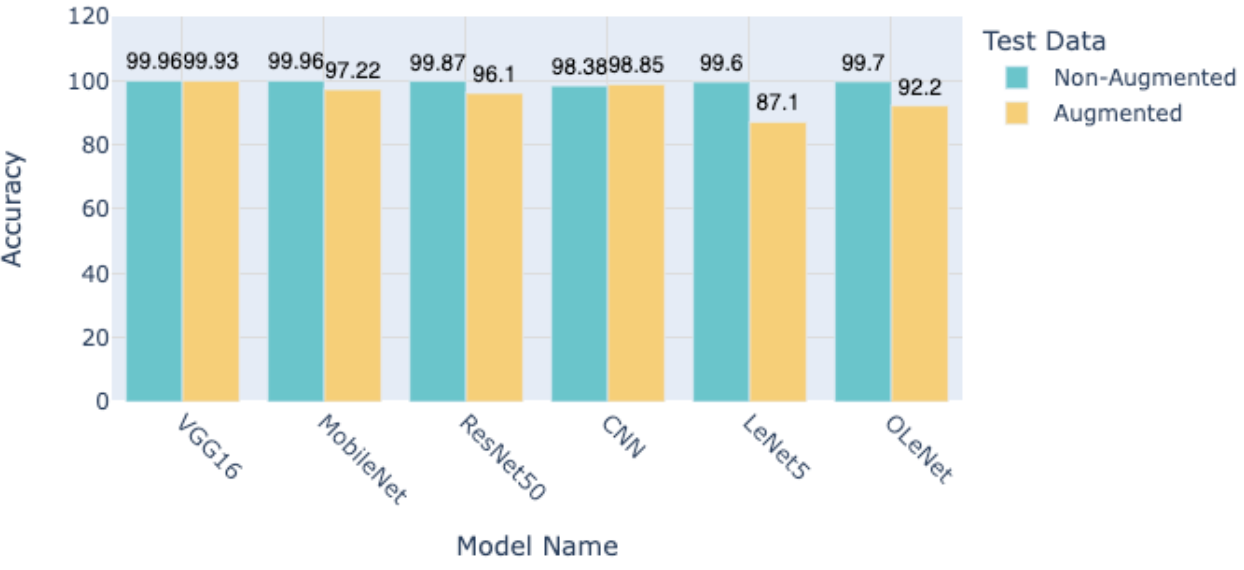
\includegraphics[scale=0.45]{Figure5_augmented_test_accuracy.png}}
\caption{Comparison of Test Accuracy Between Non-Augmented and Augmented}
\label{table}
\end{figure}

\section{Discussion & Future Improvement} 
This project showed that additional convolutional layers enhanced spatial invariance to identify key features of cracks, and early stopping could be used to save training time. As shown in results, all models appeared to have achieved high accuracies of at least 98 percent in non-augmented test, and at least 87 percent in augmented test, where VGG-16 performed the best in terms of test accuracy. Even though shallower networks such as MobileNet, LeNet5 and OLeNet were less memory intensive with less number of parameters, deeper networks such as VGG-16 performed better in accuracy; but OLeNet was able to reach minimum loss the fastest with slightly less accuracy. In comparison, MobileNet with fewer parameters performed almost as well as VGG-16. Despite the good performance, loss and accuracy graphs during model training indicated that almost all models were underfitting. There are two possible explanations for the validation set to perform as well as the training set: 1) the models were underfitting or, 2) the dataset is too simple with little variation. Another flaw with the methodology presented in this project is utilizing the augmented data to evaluate test accuracy. A reason for better than expected test accuracy with the augmented images was due to data leakage, where the augmented images used as test set were not augmented from the split test set from the non-augmented data. In addition, this project taught the important lesson that augmented images should be strictly used in model training and not testing. As the image data used in this project was zoomed in, future works should include zoomed out surface crack images that include more building exposure. In addition, video recording is another important source of data in the industry, models could also be tested in real world applications to scan for surface cracks using drones. In summary, this project further proved that OLeNet is a more optimized version of LeNet5, and that OLeNet and MobileNet can be considered in small application deployments.


\begin{thebibliography}{00}
\bibitem{b1} C.V. Dung, and L.D. Anh (2019), “Autonomous concrete crack detection using deep fully convolutional neural network,” Autom Constr., vol.99, pp. 52-58, 2019.
\bibitem{b2} M.M.M. Islam, and J-M Kim, “Vision-based autonomous crack detection of concrete structures using a fully convolutional encoder–decoder network,” Sensors, 19(19), 4251, 2019.
\bibitem{b3} I. Abdel-Qader, O. Abudayyeh, and M.E.Kelly, “Analysis of edge-detection techniques for crack identification in bridges,” J Comput Civ Eng, vol. 17, pp. 255–263, 2003.
\bibitem{b4} G. Li, X. Zhao, K. Du, F. Ru, and Y. Zhang, “Recognition and evaluation of bridge cracks with modified active contour model and greedy search-based support vector machine,” Autom Constr, vol. 78, pp. 51–61, 2017.
\bibitem{b5} Y.J. Cha, W. Choi, G. Suh, S. Mahmoudkhani, and O. Buyukozturk, “Autonomous structural visual inspection using region-based deep learning for detecting multiple damage types,” Comput Aided Civ Infrastruct Eng., 2017.
\bibitem{b6} D. Seichter, M. Eisenbach, R. Stricker, and H.-M. Gross, “How to improve deep learning based pavement distress detection while minimizing human effort,” 2018 IEEE 14th International Conference on Automation Science and Engineering (CASE), Aug. 2018.
\bibitem{b7} Y.-J. Cha, W. Choi, and O. Büyüköztürk, “Deep learning-based crack damage detection using convolutional neural networks,” Computer-Aided Civil and Infrastructure Engineering, vol. 32, no. 5, pp. 361–378, 2017.
\bibitem{b8} L. Zhang, F. Yang, Y.D. Zhang, and Y. J. Zhu, “Road Crack Detection Using Deep Convolutional Neural Network,” 2016 IEEE International Conference on Image Processing (ICIP), 2016.
\bibitem{b9} B. Kim, N. Yuvaraj, K.R.S. Preethaa, R.A. Pandian, “Surface crack detection using deep learning with shallow CNN architecture for enhanced computation,” Neural Computing and Applications, Jan. 2021.
\bibitem{b10} A.G.Howard, M. Zhu, B. Chen, D. Kalenichenko, W. Wang, T. Weyand, M. Andreetto, and H. Adam, “MobileNeta: Efficient Convolutional Neural Networks for Mobile Vision Applications,” n, arXiv:1704.0486 [cs.CV], Apr. 2017.
\end{thebibliography}
\vspace{14pt}


\end{document}
